\chapter{Submission Tool for Lecturers}
\label{Kapitel Aufruf}
The lecturer interface can be opened under cis.technikum-wien.at/My CIS/Bachelor's and Master's Thesis Submission.

\section{Overview List of the Supervised Theses}
In the overview list (see Fig. \ref{abgabetool_uebersichtsliste}) you will find all the Bachelor's and Master's theses for which you are the supervisor (summarized under project work as an umbrella term in the FAS, hence the name project work submission), and whose authors are still active.

\begin {figure}
	\centering
	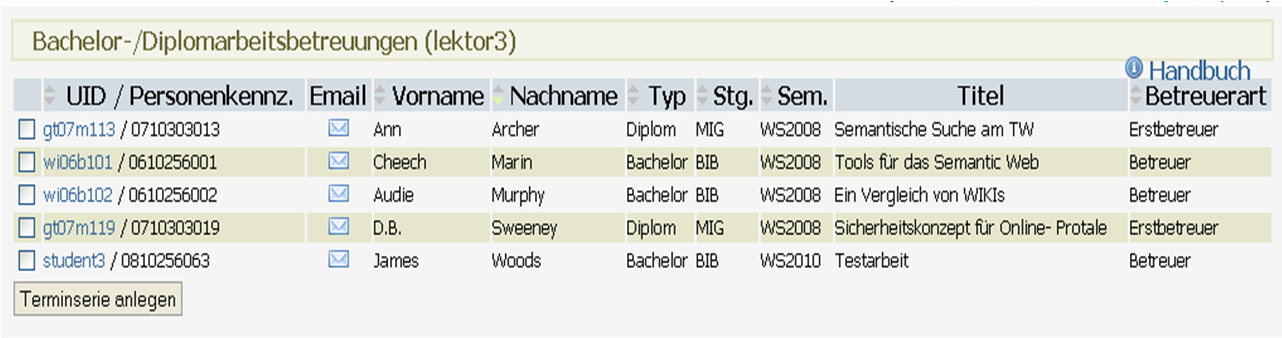
\includegraphics[width=1.0\textwidth]{abgabetool_uebersichtsliste}
	\caption{Overview List of the Supervised Theses}
	\label{abgabetool_uebersichtsliste}
\end {figure}

\subsection{Viewing the Deadline Overview}
By clicking on the UID of the student in the second column of the overview list (see Fig. \ref{abgabetool_terminverwaltung}), you can view the deadline details at the bottom portion of the page.

\subsection{Emailing Students}
By clicking the letter icon in the third column, the email client will open and fields for the recipient and sender addresses as well as the subject \textit{Bachelor's Thesis Supervision} or, \textit{Master's Thesis Supervision} will be automatically filled out.

\subsection{Setting Deadlines for Multiple Students}
It is also possible to set a deadline for multiple students at once. To do this, the relevant rows must first be marked by clicking on the checkbox in the first column. Afterwards, clicking on the button \textit{Create New Deadline Series} will open a form in the bottom portion of the browser window. The appointment is then entered here and by clicking \textit{Save} the deadline is saved for all the previously selected students.

\subsection{Opening the Instructions}
On the right side next to the heading \textit{Bachelor's/Master's Thesis Supervision} you will find a blue icon with a white i in the middle. Simply click on this symbol to open the instructions as a pdf file.

\section{Deadline Overview}

\begin {figure}
	\centering
	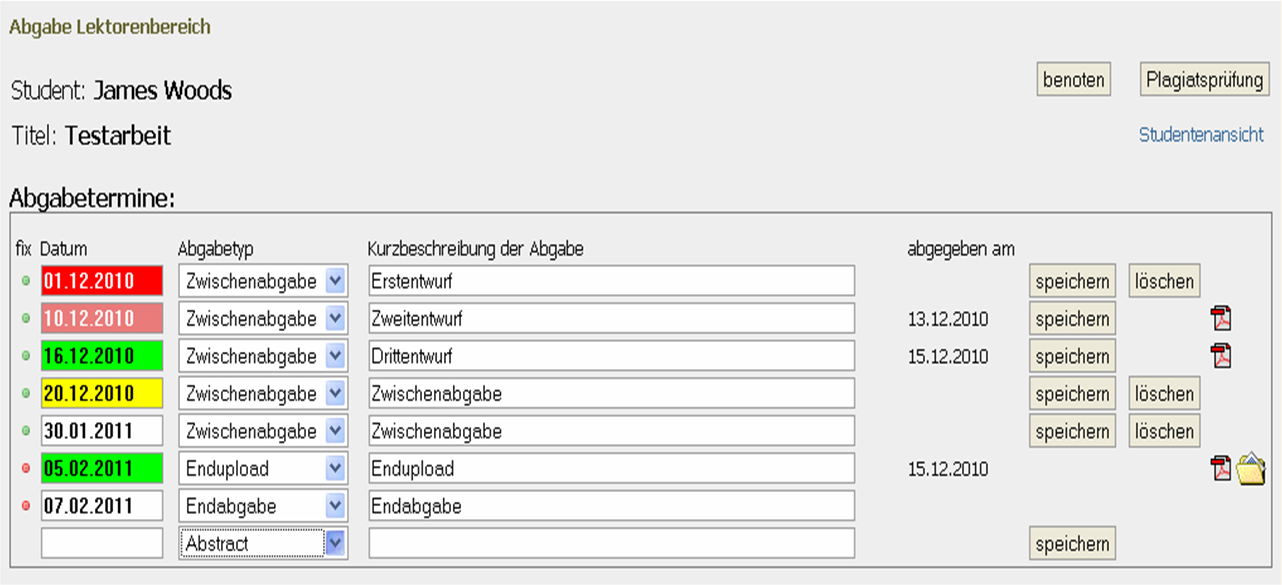
\includegraphics[width=1.0\textwidth]{abgabetool_terminverwaltung}
	\caption{ Overview and Management of Deadlines}
	\label{abgabetool_terminverwaltung}
\end {figure}

\subsection{Entering and Editing Deadlines}

\begin{itemize}
	\item Entering a Deadline: At the bottom of the list you will find a blank line with only the drop-down menu \textit{Submission Type}. You can use this line to enter new deadlines. Enter a date, select the submission type and enter a short description of the submission. Finally, click on the button \textit{Save} to save the new deadline.
	\item Changing a Deadline: Deadlines can be changed by entering the new date in the relevant line and then clicking on \textit{Save}.
	\item Deleting a Deadline: You can delete a deadline by clicking on the \textit {Delete} button. It is no longer possible to delete a deadline if a submission has already been made.
	
	\info{The student is notified by email for all three actions.}
	\item the administrative office can assign fixed deadlines which can be recognized by the red bullet under \textit{fixed}. Once the deadline has passed, the student will no longer be able to upload their submission. If something should still need to be uploaded, the student must ask the administrative assistant to correct the deadline.
	
	\info{You can only edit and delete deadlines that you have created.}
\end{itemize}

\subsection{Color Code}

\begin{itemize}
	\item White:	"'Normal"' deadline
	\item Yellow:	Deadline within the next 12 days
	\item Red:	Deadline expired
	\item Green:	Submission has been made
	\item Light Red: Submitted after the deadline 
\end{itemize}

\subsection{Downloading Submissions and Viewing Additional Data}
Clicking on the 
\includegraphics{icon_pdf} symbol will open a dialog box to save or view the submission for that deadline.
For the final submission, the student must enter additional data for the publication database. This data should be checked before carrying out the grading by clicking on the 
\includegraphics{icon_ordner_endabgabe} symbol.

\subsection{Grading}
At the top right of the deadline overview you will find the \textit{Grading} button which opens the form for grading Bachelor's and Master's theses. The data already available, such as student data, the title of the thesis and name of the reviewer, are already filled out. All that still has to be entered is the verbal descriptions of the partial grade and the points for the sections. The points awarded will be used to immediately calculate the grade based on the formula listed on the form. 

Finally, the form is printed out, signed and submitted to the administrative assistant.

\subsection{Link to the Plagiarism Check}
You will find the link to the website for the plagiarism check next to the button for the grading form. The submitted thesis can be uploaded here.

\subsection{Student View}
Below the link to the plagiarism check, you will see a link for the student view.
The submission is displayed here in the student view. You can also upload student theses from here.

\subsection{Deadline Overview for all Deadlines}
Below the list of students, it is possible to create a list of all deadlines for the supervised students. This list shows all future deadlines.

\subsection{Display Old Theses}
You can view the deadlines and theses from past students you have supervised by clicking on the link "'Show all supervised theses"' which is located below the list of students. In addition to the currently supervised theses, the list will then also display the theses that have already been graded.
